\chapter{Previous Work and Data Exploration}
\label{ch:previous_work_data}

This work seeks to compare methods proposed and corresponding results presented by Yang et al. \cite{shaanxi_publication,hainan_publication} and Hâncean et al. \cite{hancean2022occupations}. As alluded to in chapter \ref{ch:Introduction}, static network modelling, relational event modelling and relational hyperevent modelling will be compared against each other. These three methods will be applied to five different datasets. One is from Bucharest, Romania, which has already been analysed using relational hyperevent models by Hâncean et al. \cite{hancean2022occupations}; three are from Yunnan, Hainan and Shanxi, China, which have all been analysed using static network models by Yang et al. \cite{hainan_publication,shaanxi_publication}; the final dataset comprises records from all of China, and has, to the knowledge of the author, not been analysed at the time of writing this.

All the Chinese datasets are structures in the same basic manner, where records name the person who is being registered as a positively tested case, henceforth also referred to as referee; the person who is being nominated as a contact (if any), henceforth also referred to as referral; as well as covariates for referee and referral. Thus, one row equals one case contact nomination. Refer to table \ref{tab:china_data_structure} for an example. For these datasets, referees and referrals have all been tested positive for the virus.

The Romanian dataset, in contrast, consists of two tables, where one table contains all contact nominations akin to the Chinese ones, and one table contains information on positively tested patients. The patient information table contains all referees, but not all referrals, meaning that not all registered individuals were tested positive. 
To express this formally, let $A$ be the set of referees, $B$ be the set of referrals, and $P$ be the set of positively tested patients. For the Yunnan, Hainan, Shanxi and China dataset, it is $P = A \cup B$; for the Bucharest dataset, it is $A \subset P$, $B \not\subset P$, $P = A \cup X$, where $X = B_1 \cup B_2; B_1 \subset P, B_2 \not\subset P$.

\begin{table}
	\begin{tabularx}{\linewidth}{XXXXX}
		\hline
		\textbf{Timestamp} & \textbf{Referee} & \textbf{Referral} & \textbf{Referee covars [...]} & \textbf{Referral covars [...]} \\
		\hline
		2020-06-01 & p10 & p14 & ... & ... \\
		2020-06-01 & p10 & p17 & ... & ... \\
		2020-06-03 & p12 & - & ... & ... \\
		$\cdots$ & & & & \\
	\end{tabularx}
	\caption{General structure of the Chinese datasets. One row is equal to one contact nomination. Rows where the referral is empty mean there was no person nominated as contact by the referee. In this example, patient p10 nominated persons p14 and p17 as contacts, who themselves have also been tested positive. Patient p12, meanwhile, has not named anyone as a social contact.}
	\label{tab:china_data_structure}
\end{table}

\section{Yunnan Dataset}
\label{sec:yunnan_data}

\paragraph{Dataset overview} This dataset contains COVID case information from the province of Yunnan in southern China \cite{hainan_data}. There are 171 entries, with dates ranging from 2020-01-17 to 2020-02-16, i.e. this dataset is from the very early stages of the pandemic. The patient covariates deemed to be relevant are age, gender, and whether they are relatives of other confirmed cases listed in the dataset. All covariates are also listed in table \ref{tab:yunnan_hainan_covariates}.

\begin{table}
	\begin{minipage}{.45\linewidth}
		\begin{tabularx}{\linewidth}{L{.4\linewidth}L{.6\linewidth}}
			\hline
			\textbf{Covariate} & \textbf{Description}\\
			\hline
			Date & Date when the case was confirmed/reported\\
			Gender & Male/Female\\
			Age & In years\\
			Relatives & Whether the patient is a relative of previously recorded cases\\
			\hline
		\end{tabularx}
		\caption{Relevant covariates for the Yunnan and Hainan datasets}
		\label{tab:yunnan_hainan_covariates}
	\end{minipage}
	\hfill
	\begin{minipage}{.45\linewidth}
		\begin{tabularx}{\linewidth}{L{.4\linewidth}L{.6\linewidth}}
			\hline
			\textbf{Covariate} & \textbf{Description}\\
			\hline
			Date & Date when the case was confirmed/reported\\
			Gender & Male/Female\\
			Age & In years\\
			Hukou & Place of residence\\
			Relatives & Whether the patient is a relative of previously recorded cases\\
			\hline
		\end{tabularx}
		\caption{Relevant covariates for the Shanxi dataset}
		\label{tab:shanxi_covariates}
	\end{minipage}
	\begin{tabularx}{\linewidth}{L{.4\linewidth}L{.6\linewidth}}
		\hline
		\textbf{Covariate} & \textbf{Description}\\
		\hline
		Date & Date when the case was confirmed/reported\\
		Gender & Male/Female\\
		Age & In years\\
		Place of residence & \\
		Place and event & Activity where infection might have happened\\
		Symptom & The patient's symptoms\\
		Symptom severity & \\
		Place of admission & Where the patient was recorded by health authorities \\
		\hline
	\end{tabularx}
	\caption{Relevant covariates for the China dataset}
	\label{tab:china_covariates}
	\begin{tabularx}{\linewidth}{XXXXXX}
		\hline
		\textbf{Dataset} & \textbf{Age} & \textbf{Gender} & \textbf{Residence} & \textbf{Relatives} & \textbf{Degree}\\
		\hline
		Yunnan & $41\pm18$ & $\approx$ & - & $0.51$ & $1.3\pm3.2$\\
		Hainan & $48\pm17$ & $\approx$ & - & $0.46$ & $1.5\pm1.8$\\
		Shanxi & $46\pm16$ & $>men$ & Xian & $0.37$ & $0.99\pm1.3$\\
		China & $42\pm18$ & $>men$ & Xian & - & $3.6\pm18$\\
		\hline
	\end{tabularx}
	\caption{Comparison of covariates between datasets (where applicable). \emph{Gender} states which sex is more common, or whether they are roughly equal. \emph{Residence} is the most common value. \emph{Relatives} specifies the ratio of cases where relatives were recorded previously.}
	\label{tab:cov_comp}
\end{table}

Of the 171 individuals who have been confirmed positive, 114 cases have named no contacts at all, 25 have named one contact, eleven have named two contacts, and 21 have named three contacts or more. 58 and 62 cases are female and male, respectively; this information has not been recorded for the remaining 51 patients. This suggests neither sex is more susceptible to the virus. The average age of patients is $41\pm18$, with a 25 percentile of 26 and a 75 percentile of 54, meaning patients are mostly younger or middle-aged. From the 60 cases where this information is available, 31 are family members of other patients present in the dataset. 

\paragraph{Network analysis}
As previously mentioned, this dataset was analysed by Yang et al. using network modelling \cite{hainan_publication}. In their work, they determined the effect of the aforementioned patient covariates like age and gender, as well as the following network effects:
\begin{itemize}
	\item degree centrality: a node-specific centrality measure, which is equal to the number of edges connected to a node $i$. Higher-degree nodes are therefore deemed more central, i.e. important, in the network \cite{golbeck}. In the context of case contact networks, these are the patients who nominate more contacts than average.
	\item betweenness centrality: a node-specific centrality measure, which for three nodes $i,j,k$ measures the ratio of the number of shortest paths from $j$ to $k$ that go through $i$ to the total number of shortest paths from $j$ to $k$. Nodes with a high betweenness centrality are nodes that facilitate the flow of information in the network, and are therefore deemed more central, i.e. important \cite{golbeck}. In the context of case context networks, these are the patients who are likely to have transmitted the virus from one cluster of patients to another.
	\item pagerank centrality: a node-specific centrality measure based on eigenvector centrality. It is computed by performing random walks on the network and measuring the likelihood to arrive at a node $p_i$ for all nodes. Nodes with a high pagerank centrality are frequently pointed at, and are therefore deemed more central, i.e. important \cite{gleich_pagerank}. In the context of case contact networks, these are patients who have been nominated as contacts more often than average.
	\item component size: connected components are sets of nodes in a network which are strongly connected, but have no outside connected, i.e. form a coherent and isolated community. In the context of case contact networks, these represent infection clusters, and the investigation of the size of these clusters can yield insights into how the virus tends to spread.
\end{itemize} They report an average degree centrality of $1.3\pm3.2$, an average betweenness centrality of $0\pm0$, and an average pagerank centrality of $0.0058\pm0.0055$. Furthermore, three of 18 connected components comprise of more than three nodes \cite{hainan_publication}. 

According to Yang et al., the zero value for betweenness centrality indicates that transmission of the virus from patient to patient happened near-simultaneously and in clusters, rather than in long transmission chains; A maximum pagerank score of 0.0221 compared to the mean value of $0.0058\pm0.0055$ means that ties are distributed unequally among patients, with a small number of patients being associated with most contact nominations. Furthermore, they write that the large fraction of nodes without ties is due to those patients hailing from another state, which made tracing of their contacts difficult; however, it isn't exactly stated why contact tracing was not possible for this group. The development of the case contact network over time was also analysed, albeit on a coarse level, where states of the network at three distinct points in time (start, middle and end point of the time period) were compared. Findings suggest that early cases were mostly imported from other provinces, since those mostly had no associated contacts, while local infection clusters only emerged in the later stages \cite{hainan_publication}. 

\section{Hainan Dataset}
\label{sec:hainan_data}

\paragraph{Dataset overview} This dataset contains COVID case information from the province of Hainan \cite{hainan_data}, which is the southernmost province of China. It was released in tandem with the Yunnan dataset, and therefore patient covariates are the same. There are 162 entries, with dates ranging from 2020-01-22 to 2020-02-14, i.e. this dataset is also from the early stages of the pandemic. Of the 162 confirmed cases, 71 have named no contacts, 27 have named one contact, 21 have named two contacts, and 43 have named three contacts or more. 

84 and 78 cases are female and male, respectively. An average age of $48\pm17$, a 25 percentile of 36 and a 75 percentile of 62 mean that the patients in this dataset are from an older age group compared to the Yunnan data. 75 out of 162 patients are family members of previously recorded cases.

\paragraph{Network analysis} This dataset was analysed by Yang et al. using the same methodology outlined in section \ref{sec:yunnan_data}. They report an average degree centrality of $1.51\pm1.79$, an average betweenness centrality of $0\pm0$, and an average pagerank centrality of $0.0062\pm0.0043$. Ten out of 27 connected components are comprised of more than three nodes \cite{hainan_publication}. 

Interpretation of these numbers is similar to the Yunnan network. The zero value for betweenness centrality again indicated transmission happening in clusters rather than chains, and a maximum pagerank score of 0.0189 compared to the mean $0.0062\pm0.0043$ suggests an uneven distribution of ties. However, the larger fraction of patients with contacts (57\% here vs. just 33\% in the Yunnan dataset), paired with the larger number of connected components (27 vs. 18) means that less cases were imported from other states and/or containment measures might not have been as effective (the authors state that imposed measures were largely the same for both Yunnan and Hainan provinces). Accordingly, the temporal development of the case contact network shows an earlier emergence of infection clusters \cite{hainan_publication}.

\section{Shaanxi Dataset}
\label{sec:shaanxi_data}

\paragraph{Dataset overview} This dataset contains COVID case information from the province of Shaanxi in northern China \cite{shaanxi_data}. There are 237 entries, with dates ranging from 2020-01-23 to 2020-02-16, so this dataset too is from the early stages. Relevant covariates are mostly equivalent to those of the previous two discussed sets, with the addition of the place of residence; covariates are listed in table \ref{tab:shanxi_covariates}. 

Of the 237 positively tested patients, 108 cases have named no contacts at all, 68 have named one contact, 36 have named two contacts, and 25 have named three contacts or more.  With 129 versus 108, there are slightly more men in this dataset compared to the near-equal distribution found in the previous two discussed datasets. The average age of patients is $46\pm17$, the 25 percentile is 35, and the 75 percentile is 59. Only 87 of the 237 patients are family members of previously recorded cases, suggesting that the majority of infections were transmitted from stranger to stranger rather than between family members; this is a contrast to the near-equal distribution found in the Yunnan and Hainan datasets (36.7\% vs. 51.6\% and 46.2\%, respectively). The three most common places of residence are \emph{Xian}, \emph{Ankang} and \emph{Hanzhong}.

\paragraph{Network analysis} This dataset, too, was analysed by Yang. In addition to the previously discussed network statistics, closeness centrality was also included in the analysis. Closeness centrality a node-specific centrality measure, which is defined as the reciprocal of the sum of all shortest paths for a node $i$. Nodes with a high closeness centrality are nodes that are only a few edges away from other nodes, and are therefore deemed more central, i.e. important \cite{sabidussi1966centrality}. 

Reported were an average degree centrality of $.99\pm1.3$, an average closeness centrality of $0.45\pm0.44$, and average betweenness centrality of $0\pm0$, and an average pagerank centrality of $0.0042\pm0.0035$. 12 out of 40 connected components are comprised of more than three nodes. Interpretations are analogous to the other datasets; a tie to no-tie ratio of 54\% paired with the highest number of connected components yet suggest a tendency for cluster outbreaks similar to Hainan province, a fact which the author claims is corroborated by the average closeness centrality value \cite{shaanxi_publication}.

\section{Xi'an Dataset}
\label{sec:xian_data}

\paragraph{Dataset overview} This dataset contains COVID case information from the city of Xi'an, which is located in the Shaanxi province in northern China \cite{xian_data}. There are 2050 entries; unfortunately, despite being present in the corresponding research paper, neither dates nor patient covariates were included in the referenced dataset \cite{xian_publication,xian_data}. It's important to note that the article is merely a preprint version and its status is currently under major revision. Still, this dataset may provide interesting insights in the comparison of different regions. It is stated in the paper that dates range from 2021-12-09 to 2022-01-18, i.e. this network is the first to depict a mid-pandemic time period. 

Out of the 2050 positively tested patients, 965 cases have named no contacts at all, 871 have named one contact, 132 have named two contacts, and 82 have named three contacts or more. The average age of patients is $36\pm18$, and the male-to-female ratio is 55.5\% (1118 men vs. 932 women). There is no information regarding the 25 and 75 percentiles of patient age. 

\paragraph{Network analysis} Network statistics used by Yang are degree centrality, pagerank centrality, closeness centrality, betweenness centrality, component size and triadic census; the author explains that this means the count of possible triadic structures (ref. \ref{fig:triadic_structures}) present in the graph. They report those counts to be 545,154 for the 003 configuration, 1,550,928 for the 102 configuration, 1,752 for the 201 configuration, and 0 for the 300 configuration. Yang claims that triadic census can be used to analyse the spread pattern of the virus, but unfortunately does not elaborate further on this.

Values for degree centrality, pagerank centrality, closeness centrality and betweenness centrality are $0.7\pm1.4$, $0.0005\pm0.0006$, $0.4\pm0.4$, and $3.4\pm50.6$, respectively. The value for betweenness centrality is especially interesting since it was always zero up until now. This suggests that there were more transmission chains and/or different clusters connected by a single individual, as opposed to the isolated infection clusters that can be seen in the other datasets. The author provides no interpretation for the other statistics.

There are 1291 connected components, and 82 out of those consist of more than three nodes. Since this dataset is significantly larger than the ones discussed previously, these numbers are not directly comparable. This is addressed by computing the modularity score of the networks; a reported value of 0.95 for this network vs. 0.99 for the Shaanxi network suggests these are similarly structured. This notion is further supported by the tie to no-tie ratio of 53\%.

\begin{figure}
	\centering
	\begin{subfigure}[b]{0.2\linewidth}
		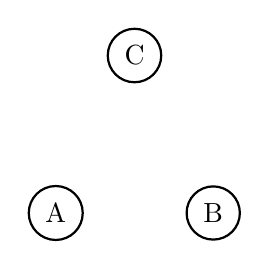
\begin{tikzpicture}
			\begin{scope}[every node/.style={circle,thick,draw}]
				\node (A) at (0,0) {A};
				\node (B) at (2,0) {B};
				\node (C) at (1,2) {C};
			\end{scope}
			
			\begin{scope}
				%\path (A) edge node {} (B);
				%\path (B) edge node {} (C);
				%\path (C) edge node {} (A);
			\end{scope}
		\end{tikzpicture}
		\caption{003 configuration}
	\end{subfigure}
	\hfill
	\begin{subfigure}[b]{0.2\linewidth}
		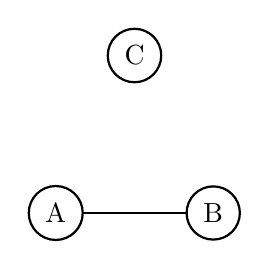
\begin{tikzpicture}
			\begin{scope}[every node/.style={circle,thick,draw}]
				\node (A) at (0,0) {A};
				\node (B) at (2,0) {B};
				\node (C) at (1,2) {C};
			\end{scope}
			
			\begin{scope}
				\path (A) edge node {} (B);
				%\path (B) edge node {} (C);
				%\path (C) edge node {} (A);
			\end{scope}
		\end{tikzpicture}
		\caption{102 configuration}
	\end{subfigure}
	\hfill
	\begin{subfigure}[b]{0.2\linewidth}
		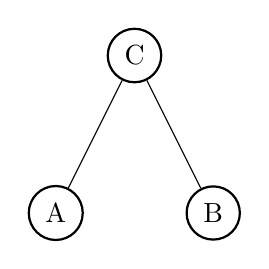
\begin{tikzpicture}
			\begin{scope}[every node/.style={circle,thick,draw}]
				\node (A) at (0,0) {A};
				\node (B) at (2,0) {B};
				\node (C) at (1,2) {C};
			\end{scope}
			
			\begin{scope}
				%\path (A) edge node {} (B);
				\path (B) edge node {} (C);
				\path (C) edge node {} (A);
			\end{scope}
		\end{tikzpicture}
		\caption{201 configuration}
	\end{subfigure}
	\hfill
	\begin{subfigure}[b]{0.2\linewidth}
		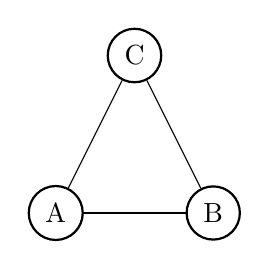
\begin{tikzpicture}
			\begin{scope}[every node/.style={circle,thick,draw}]
				\node (A) at (0,0) {A};
				\node (B) at (2,0) {B};
				\node (C) at (1,2) {C};
			\end{scope}
			
			\begin{scope}
				\path (A) edge node {} (B);
				\path (B) edge node {} (C);
				\path (C) edge node {} (A);
			\end{scope}
		\end{tikzpicture}
		\caption{300 configuration}
	\end{subfigure}
	\label{fig:triadic_structures}
	\caption{Possible triadic structures for any three nodes $A,B,C$.}
\end{figure}


\section{China Dataset}
\label{sec:china_data}

\paragraph{Dataset overview} This dataset contains COVID case information from all of China \cite{china_publication,china_data}. After preprocessing, there are 25,877 entries, with dates ranging from 2020-01-01 to 2022-08-14; therefore, this set is significantly larger than the ones discussed previously, and covers most of the pandemic. Relevant patient covariates are age, gender, residence, the location and/or activity where the patient was most likely infected, the patient's symptoms, the severity of the symptoms, and where the patient was registered by health authorities; covariates are also listed in \ref{tab:china_covariates}. The number of recorded covariates makes this dataset stand out among the others.

Out of the 25,877 confirmed cases, 20,577 have named no contacts at all, 2,995 have named one contact, 1,045 have named two contacts, and 1,260 have named three contacts or more. The mean age of patients is $42\pm18$ (information missing for 6,206 entries), with a 25 percentile of 30 and a 75 percentile of 54, meaning this dataset contains members of all age groups. 9,070 women versus 11,182 men shows a slight bias towards men (information missing for 5,625 entries). The three most common places of residence are \emph{Xi'an} (1,947), \emph{Wuhan} (1,671), and \emph{Shijiazhuang} (888) (information missing for 9,077 entries). The three most common occasions where patients were most likely infected are \emph{travel to Wuhan} (596), \emph{dinner} (360), and \emph{residence in Wuhan} (337) (information missing for 18,167 entries). The three most common symptoms are \emph{somatosensory related} (1,904), \emph{respiratory system/somatosensory related} (640), and \emph{respiratory system related} (495) (information missing for 20,142 entries). Out of the 7,061 cases where this information is available, 3,979 are classified as stable, 2,545 have mild symptoms, 405 have light symptoms, and 132 have severe symptoms. The three most common places of admission, i.e. where the patient was registered/admitted to hospital are \emph{Xi'an} (2292), \emph{Shanghai} (2079), and \emph{Guangzhou} (1398).

\paragraph{Network analysis} To the knowledge of the author, this dataset had not been analysed yet at the time of writing this.

\paragraph{A note on data quality} This dataset was compiled from 291 different data sources and although Liu et al. did a splendid job in standardising and coding the included variables, it's likely there are still some inconsistencies present in the data even after preprocessing, e.g. city names being written slightly different (Xi'an, Xian) and thus producing two unique values instead of one. Still, this should only be true for a negligible fraction of data entries, and thus not impact results in a significant manner.

\section{Bucharest Dataset}
\label{sec:bucharest_dataset}

\paragraph{Dataset overview} This dataset contains COVID case information from Bucharest, the capital of Romania \cite{bucharest_data}. It consists of 46,269 positively tested patients, of which 6,895 named at least one other person as a possible contact. Out of the 13,272 individuals nominated as contacts, 1,811 were themselves recorded as patients; therefore, this dataset differs from the others in the sense that not all named contacts were tested positive. Dates range from 2020-03-07 to 2020-11-11. Patient covariates deemed relevant are age, sex, the patient's field of work and whether the patient is active in the medical field; these are also listed in table \add{table, reference}. Out of the 46,269 positive cases and the additional 11,461 individuals who were nominated as contacts but were not themselves recorded as patients, 38,122 individuals have named no contacts at all, 15,856 have nominated one contact, 2,130 have nominated two contacts, and 1,727 patients have named three contacts or more \add{numbers don't add up, not sure why}. 

The average age of patients is $41\pm19$, with a 25 percentile of 29 and a 75 percentile of 53, meaning most are on the younger side. 21,665 males versus 24,604 females shows a slight bias towards females. Of the 6,964 patients where this information was recorded, only 186 are active in the medical field. Furthermore, a majority of patients for whom job information was recorded are not active in the labour market (6,298 out of 9,806). 

\paragraph{Network analysis} This dataset was analysed by H\^ancean et al. in two separate papers, with the first focusing on the role of age \cite{hancean2021role}, and the second addressing the impact of occupations on the spread of COVID-19 \cite{hancean2022occupations}.

\bigskip

In the first article, the authors combined patient covariates and certain network statistics into a relational hyperevent model (discussed in detail in section \ref{ch:methods}), which was then used to determine the impact of these variables on the likelihood of contact nominations. Specifically, they investigated age homophily, i.e. the average age difference between contact nominator (called \emph{referee} in the original paper) and nominees (called \emph{referrals} in the original paper); the average age of nominated contacts; sex homophily, i.e. the average sex difference between contact nominator and nominees; the average sex of nominated contacts; individual contact popularity, i.e. how often an individual is named as a contact; joint contact popularity, i.e. how often a pair of individuals have been named as contacts together; reciprocation, i.e. for any possible case contact nomination, where $i$ names $\{j,k,...,n\}$ as contacts at time $t_x$, how many individuals from $\{i,j,...,k\}$ have themselves named $i$ as a contact at a previous time $t_{x-y}$; contact activity, i.e. the number of contacts an individual has nominated before; nominations among contacts, i.e. for any possible case contact nomination, where $i$ names $\{j,k,...,n\}$ as contacts at time $t_x$, how many pairs of individuals $(j,k) \in \{j,k,...,n\}$ were involved in a contact nomination, where $j$ names $k$ as a contact, at a previous time $t_{x-y}$; and shared referee, i.e. for any possible case contact nomination, where $i$ names $\{j,k,...,n\}$ as contacts at time $t_x$, how many individuals from $\{j,k,...,n\}$ were named as contacts together with $i$ at a previous time $t_{x-y}$.

H\^ancean et al. reported the following results. The age difference between nominator and nominees is negatively associated with contact nomination likelihood, i.e. for any possible case contact nomination, where $i$ names $\{j,k,...,n\}$ as contacts, the likelihood of that contact nomination decreases with an increasing age discrepancy between nominator $i$ and nominees $\{j,k,...,n\}$; thus, there is age homophily, meaning that patients are likely to nominate contacts with an age similar to themselves. The average age of nominees is negatively associated with contact nomination likelihood, i.e. for any possible case contact nomination, where $i$ names $\{j,k,...,n\}$ as contacts, the likelihood of that contact nomination decreases with an increasing average age of the nominees $\{j,k,...,n\}$; this means that younger people are more likely to be nominated as contacts. The sex difference between nominator and nominees is positively associated with contact nomination likelihood, i.e. for any possible case contact nomination, where $i$ names $\{j,k,...,n\}$ as contacts, the likelihood of that contact nomination increases with an increasing degree of sex discrepancy between nominator $i$ and nominees $\{j,k,...,n\}$; thus, there is sex heterophily, meaning that patients are likely to nominate contacts of the opposite sex. Finally, the average sex of nominees is positively associated with contact nomination likelihood, i.e. for any possible case contact nomination, where $i$ names $\{j,k,...,n\}$ as contacts, the likelihood of that contact nomination increases with an increasing ratio of women in the nominee set $\{j,k,...,n\}$ (this is because sex was coded as male = 1 and female = 2; therefore, a higher average value across the nominee set means a higher fraction of nominees is female, while a lower average value would mean there are more males); this means that women are more likely to be nominated as contacts.

As for the network effects, the authors report these results. Individual contact popularity is negatively associated with contact nomination likelihood, i.e. for any possible case contact nomination, where $i$ names $\{j,k,...,n\}$ as contacts at time $t_x$, the likelihood of that contact nomination decreases with an increasing number of times individuals $\in \{j,k,...,n\}$ have already been named as contacts at previous times $t_{x-y}$; this means that individuals are unlikely to be named as a contact multiple times, although the authors note this is due to the nature of the dataset, where actors are very unlikely to appear more than once. Joint contact popularity is positively associated with contact nomination likelihood, i.e. for any possible case contact nomination, where $i$ names $\{j,k,...,n\}$ as contacts at time $t_x$, the likelihood of that contact nomination increases with an increasing number of pairs $(j,k) \in \{j,k,...,n\}$ who have been co-named as contacts in a previous contact nomination at time $t_{x-y}$; this means that people who are socially close are more likely to be nominated as contacts. Reciprocation is positively associated with contact nomination likelihood, i.e. for any possible case contact nomination, where $i$ names $\{j,k,...,n\}$ as contacts at time $t_{x}$, the likelihood of that contact nomination increases with an increasing number of individuals $\in \{j,k,...,n\}$ who have themselves nominated $i$ as a contact in a previous contact nomination at time $t_{x-y}$. This means nominated contacts tend to "return the favour". Contact activity is negatively associated with contact nomination likelihood, i.e. for any possible case contact nomination, where $i$ names $\{j,k,...,n\}$ as contacts at time $t_x$, the likelihood of that contact nomination decreases with an increasing number of contacts nominated by individuals $\in \{j,k,...,n\}$ in previous contact nominations at times $t_{x-y}$; this means that individuals who have previously acted as nominators are less likely to be named as contacts themselves later, which is again attributed to the nature of the dataset (see individual contact popularity). Nominations among contacts is positively associated with contact nomination likelihood, i.e. for any possible case contact nomination, where $i$ names $\{j,k,...,n\}$ as contacts at time $t_x$, the likelihood of that contact nomination increases with an increasing number of pairs $(j,k) \in \{j,k,...,n\}$ who were involved in a previous contact nomination at time $t_{x-y}$, where $j$ was the nominator and $k$ one of the nominees. This means that socially close individuals are more likely to be nominated as contacts together, in a similar fashion to joint contact popularity. Finally, shared referee is positively associated with contact nomination likelihood, i.e. for any possible case contact nomination, where $i$ names $\{j,k,...,n\}$ as contacts at time $t_x$, the likelihood of that contact nomination increases with an increasing number of individuals $j \in \{j,k,...,n\}$ who have been involved in a previous contact nomination at time $t_{x-y}$, where $i$ and $j$ were named as contacts together. This again hints at the influence of social closeness \cite{hancean2021role}.

\bigskip

In the second article, H\^ancean et al. analysed the dataset again, in a similar fashion, this time placing the focus on the role of occupations in the spread of COVID-19. For this, they added the following patient covariates to the model. Whether the individual was unemployed at the time of registration; whether the individual was employed in the private or public sector; whether the individual was employed in the medical sector; whether the individual was active in the labour market, i.e. either employed or employable; and the individual's age group, i.e. minor, adult, or pensioner.

Specifically, the authors investigated age homophily; the average age of nominated contacts; the age of the nominator; sex homophily; the average sex of nominated contacts; the sex of the nominator; the fraction of nominees active in the public sector; whether the nominator is active in the public sector; the fraction of nominees active in the medical sector; whether the nominator is active in the medical sector; active working force difference, i.e. the fraction of nominees who are either employed or employable, compared to whether the nominator is active in the workforce or not; the fraction of active nominees; whether the nominator is active in the workforce; individual contact popularity; joint contact popularity; reciprocation; in-degree of the nominator, i.e. for any possible contact nomination, where $i$ names $\{j,k,...,n\}$ as contacts at time $t_x$, how many times the nominator has himself been named as a contact at a previous time $t_{x-y}$; out-degree of the nominees, i.e. for any possible contact nomination, where $i$ names $\{j,k,...,n\}$ as contacts at time $t_x$, how many times contacts $j \in {j,k,...,n}$ have themselves acted as contact nominators at a previous time $t_{x-y}$; nominations among contacts; and shared referee;

The following results were reported regarding patient covariates. Nominator age is positively associated with contact nomination likelihood, i.e. for any possible contact nomination, where $i$ names $\{j,k,...,n\}$ as contacts, the likelihood of that contact nomination increases with an increasing age of $i$; this means that older people are more likely to contract COVID-19 and appear as nominators. There is no significant effect of the average age of nominees on contact nomination likelihood, i.e. for any possible contact nomination, where $i$ names $\{j,k,...,n\}$ as contacts, the average age of $\{j,k,...,n\}$ does not influence the likelihood of that contact nomination. The age difference between nominator and nominees is negatively associated with contact nomination likelihood, i.e. for any possible contact nomination, where $i$ names $\{j,k,...,n\}$ as contacts, the likelihood of that contact nomination decreases with an increasing age discrepancy between nominator $i$ and nominees $\{j,k,...,n\}$; thus, there is age homophily, as was found in the first paper. Nominator sex is positively associated with contact nomination likelihood when not controlling for network effects, i.e. for any possible contact nomination, where $i$ names $\{j,k,...,n\}$ as contacts, the likelihood of that contact nomination increases with if $i$ is female. The average sex of nominees is positively associated with contact nomination likelihood, i.e. for any possible contact nomination, where $i$ names $\{j,k,...,n\}$ as contacts, the likelihood of that contact nomination increases with an increasing ratio of women in the nominee set $\{j,k,...,n\}$ (again, sex was coded as male = 1 and female = 2); this means that women are more likely to be nominated as contacts, corroborating the authors' previous findings. The sex difference between nominator and nominees is positively associated with contact nomination likelihood, i.e. for any possible contact nomination, where $i$ names $\{j,k,...,n\}$ as contacts, the likelihood of that contact nomination increases with an increasing degree of sex discrepancy between nominator $i$ and nominees $\{j,k,...,n\}$; thus, there is sex heterophily, as was in the preceding article. Whether the nominator is working in the public sector is negatively associated with contact nomination likelihood, i.e. for any possible contact nomination, where $i$ names $\{j,k,...,n\}$ as contacts, the likelihood of that contact nomination decreases if the nominator $i$ works in the public sector; this means that people active in the public sector are less likely to contract COVID-19 and appear as nominators. The fraction of nominees working in the public sector is negatively associated with contact nomination likelihood, i.e. for any possible contact nomination, where $i$ names $\{j,k,...,n\}$ as contacts, the likelihood of that contact nomination decreases with an increasing number of nominees who are active in the public sector; this means that people who work in the public sector are also less likely to be named as contacts. Whether the nominator is active in the medical sector has no significant effect on contact nomination likelihood. The fraction of nominees active in the medical sector is negatively associated with contact nomination likelihood, i.e. for any possible contact nomination, where $i$ names $\{j,k,...,n\}$ as contacts, the likelihood of that contact nomination decreases with an increasing number of nominees who are active in the medical sector; this means that people who work in the medical sector are less likely to be named as contacts.  Whether the nominator is active in the workforce is positively associated with contact nomination likelihood, while the fraction of nominees who are active in the workforce is negatively associated with contact nomination likelihood, i.e. for any possible contact nomination, where $i$ names $\{j,k,...,n\}$ as contacts, the likelihood of that contact nomination increases if the nominator $i$ is active in the workforce, and decreases with an increasing number of nominees $\{i,j,...,k\}$ who are active in the workforce; this means that being either employed or employable increases the chance to contract COVID-19 and appear as a nominator, and decreases the chance to be named as contact. Accordingly, the active working force difference is positively associated with contact nomination likelihood, i.e. for any possible contact nomination, where $i$ names $\{j,k,...,n\}$ as contacts, the likelihood of that contact nomination increases with an increasing discrepancy of being active in the workforce between nominator $i$ and nominees $\{j,k,...,n\}$; this means that active people are more likely to nominate non-active individuals as contacts, and thus, there is an anti-homophily. 

As for the network effects, results were the following. Individual contact popularity is negatively associated with contact nomination likelihood; joint contact popularity is positively associated with contact nomination likelihood; reciprocation is positively associated with contact nomination likelihood; nominations among contacts is positively associated with contact nomination likelihood; shared referee is positively associated with contact nomination likelihood. These results corroborate findings from the previous article, and thus, interpretations are equivalent. Both the in-degree of the nominator and the out-degree of the nominees are negatively associated with contact nomination likelihood, i.e. for any possible contact nomination, where $i$ names $\{j,k,...,n\}$ as contacts at time $t_x$, the likelihood of that contact nomination decreases with an increasing number of previous contact nominations at a time $t_{x-y}$, where $i$ was named as a contact, and also decreases with an increasing number of previous contact nominations at a time $t_{x-y}$, where an individual $j \in \{j,k,...,n\}$ acted as a nominator \cite{hancean2021role,hancean2022occupations}. 

\paragraph{A note on data availability and ethical considerations} Although a fair number of research on the topic of contact tracing data have been published (e.g. \add{CITE}), general data availability was rather restricted at the time of writing this. Many datasets were either only available upon request to the respective author or outright unavailable, presumably due to privacy considerations. Some were even behind paywalls. Due to this, four of the five datasets used in this work originate from China, where such data is widely available and was regularly published by local health authorities during the pandemic. Since all data records have been pseudonymised, there should be no ethical concern regarding privacy violation.